\documentclass[journal]{IEEEtran}

\usepackage[T1]{fontenc}
\usepackage{microtype}

\usepackage{amsmath,amssymb}
\usepackage{booktabs}
\usepackage{array}
\usepackage{graphicx}
\usepackage{url}
\usepackage{xurl}
\usepackage{multirow}
\usepackage{float}
\usepackage{enumitem}

% Typesetting adjustment to prevent margin overflow warnings
\emergencystretch 3em

% =========================================================
% FRONT MATTER
% =========================================================

\begin{document}

\title{A Sustainable Hybrid QKD--PQC Security Architecture for
Quantum-Resilient Residential IoT}

\author{Prakash Suryawanshi%
\thanks{P.~Suryawanshi is the Founder and Director of Qodeigence Infocircle
Private Limited, Maharashtra, India (e-mail: prakashsurywanshi1@live.com).}}

\maketitle

\begin{abstract}
The rapid proliferation of Internet of Things (IoT) technologies across residential
environments creates a security problem that is fundamentally intertwined with computing
sustainability. Constrained smart home nodes operate under strict energy, memory,
computational, and bandwidth bounds while facing the threat posed by quantum
cryptanalysis via Shor's algorithm. 

This paper proposes a sustainable hybrid security architecture for quantum-resilient
residential IoT. The architecture introduces an edge-centric Quantum-Safe Home Security
Gateway (QHSG) that structurally isolates security-intensive key-management operations
from high-volume application data streams. Last-mile access-node Quantum Key Distribution
(QKD) key material is incorporated where optical infrastructure is available, while
standardized Post-Quantum Cryptography (PQC) mechanisms provide a deployable security
path over conventional networks. Bulk application data is secured using authenticated
symmetric encryption.

The principal contribution is a security--sustainability framework that formalizes
computational energy, radio communication overhead, 6LoWPAN fragmentation penalties,
and adaptive key-refresh intervals as explicit design parameters. We validate the
architecture through a benchmark-calibrated empirical simulation modeling ARM Cortex-M4
leaf endpoints across network scales from $N=10$ to $N=500$ devices, augmented by
protocol-level validation of the 6LoWPAN fragmentation model in COOJA and by
symbolic formal verification of the key-lifecycle and refresh-policy security
invariants in ProVerif. The results, obtained at an IEEE 802.15.4 physical rate of $250\,\text{kbps}$ with
radio constants anchored to device datasheets, demonstrate that direct leaf-node PQC
deployment increases endpoint key-negotiation energy by $108.4\%$ over classical handshakes
due to transmission and fragmentation of large lattice keys. In contrast, the proposed
QHSG-mediated hybrid architecture offloads asymmetric encapsulation to the gateway,
reducing endpoint key-management energy by $96.8\%$ relative to standalone PQC and
$93.3\%$ relative to classical ECDH, establishing a sustainable path toward post-quantum
resilience in battery-driven smart homes. A sensitivity analysis across the full
plausible range of platform parameters confirms that these conclusions are robust.
\end{abstract}

\begin{IEEEkeywords}
sustainable computing, quantum computing, post-quantum cryptography, quantum key
distribution, Internet of Things, smart home, energy efficiency.
\end{IEEEkeywords}

% =========================================================
% 1. INTRODUCTION
% =========================================================

\section{Introduction}

Residential environments are increasingly becoming dense, distributed computing systems
composed of cameras, smart locks, lighting controllers, thermostats, energy meters, motion
sensors, appliances, and smart controllers. These devices continuously process and exchange
telemetry and actuation commands through local personal area networks (PANs), edge routers,
and remote cloud servers \cite{nist8259a,nist8259,lin2017survey}.

The security requirements of residential IoT deployments are critical. Compromised telemetry
can reveal physical occupancy patterns, behavioral routines, private audio conversations,
and access authorization states \cite{alrawi2019sok}. A compromised surveillance stream directly
violates resident privacy, while compromised smart locks or safety actuators lead to
tangible physical hazards.

However, security cannot be designed independently of computing sustainability. Leaf IoT nodes
frequently operate on constrained embedded microcontrollers (MCUs) characterized by limited
clock frequencies, narrow RAM buffers, and battery power sources \cite{gungor2021sustainable,minerva2015towards}.
Cryptographic operations draw power from limited batteries and generate network traffic that
consumes energy across wireless transceivers \cite{khan2020energy}.

This tension is exacerbated by the transition toward quantum-resilient cryptographic
standards. Shor's algorithm provides a polynomial-time solution for integer factorization
and discrete logarithms, rendering classical public-key mechanisms (e.g., RSA and ECC)
vulnerable to cryptanalytically relevant quantum computers \cite{shor,bernstein2017post}.
Furthermore, the prevalent ``harvest now, decrypt later'' attack model implies that
adversaries can intercept and archive encrypted smart-home traffic today, awaiting quantum
advancements to compromise sensitive historical payloads \cite{mosca,mavroeidis2018impact}.

To address algorithmic vulnerabilities on classical hardware, NIST standardized Post-Quantum
Cryptography (PQC) in 2024 through FIPS 203 (ML-KEM), FIPS 204 (ML-DSA), and FIPS 205
(SLH-DSA) \cite{nist203,nist204,nist205}. Quantum Key Distribution (QKD) provides a
complementary, physics-based mechanism to establish information-theoretically secure key
material via quantum optics \cite{bb84,scarani,pirandola,etsi}. However, deploying dedicated
single-photon QKD receivers to residential leaf nodes is economically infeasible and
operationally unsustainable. Similarly, direct execution of lattice-based PQC algorithms
on constrained endpoints introduces communication overheads that overwhelm low-power radio
transceivers \cite{kannwischer2020pqm4,alkim2016kyber}.

Deploying quantum resilience in smart homes is therefore an architectural sustainability
challenge. An architecture that increases endpoint radio duty cycles will exhaust battery
reserves, leading to premature battery discard and increased electronic waste
\cite{marcu2020lifecycle}.

This paper addresses the following research question:
\begin{quote}
How can QKD and PQC be integrated into residential IoT architectures to deliver quantum
resilience while minimizing endpoint computational, communication, and energy overheads?
\end{quote}

The proposed solution is an edge-centric architecture centered on a mains-powered
Quantum-Safe Home Security Gateway (QHSG). The QHSG aggregates external optical QKD key
streams from last-mile access loops, negotiates post-quantum handshakes with cloud services,
and provisions lightweight symmetric key sessions to leaf nodes.

% =========================================================
% 2. RESEARCH GAP AND MOTIVATION
% =========================================================

\section{Research Gap and Motivation}

Existing studies examine post-quantum cryptography, QKD networks, IoT security, and green
computing as isolated domains \cite{kaur2021sustainable,campagna2020quantum}. However,
smart residential systems require balancing security against tight resource limits.

Three specific observations motivate this research:
\begin{enumerate}
    \item \textbf{Disproportionate Radio Overhead of PQC:} While lattice-based key
    encapsulation mechanisms (e.g., ML-KEM-768) compute rapidly on 32-bit MCUs, their public
    keys and ciphertexts exceed $1\,\text{KB}$ \cite{kannwischer2020pqm4}. On IEEE 802.15.4
    links with a $127\,\text{byte}$ Maximum Transmission Unit (MTU), a single post-quantum
    handshake triggers extensive 6LoWPAN packet fragmentation, increasing transmission energy
    by orders of magnitude \cite{montenegro2007transmission}.
    \item \textbf{Infeasibility of Leaf-Node QKD:} Direct QKD deployment requires specialized
    optical fiber, single-photon avalanche detectors, and active polarization alignment
    \cite{scarani,diamanti2016practical}. Equipping residential sensors with quantum optical
    hardware is cost-prohibitive and energy-inefficient.
    \item \textbf{Failure to Decouple Negotiation from Encryption:} Cryptographic protection
    does not require running asymmetric post-quantum handshakes for every individual data frame.
    Key establishment can be separated from continuous, high-volume bulk data encryption
    \cite{barker2020recommendation}.
\end{enumerate}

The research gap addressed by this paper comprises:
\begin{enumerate}[label=(\roman*)]
    \item The absence of a gateway-centric architecture that combines optical access-node
    QKD with standardized PQC for residential IoT;
    \item The lack of an explicit security--sustainability formulation accounting for
    endpoint compute, packet fragmentation overhead, and gateway offloading;
    \item The absence of comparative benchmark-driven evaluations quantifying the energy
    penalties of quantum-safe migration in smart home networks.
\end{enumerate}

% =========================================================
% 3. CONTRIBUTIONS
% =========================================================

\section{Contributions}

The principal contributions of this paper are:
\begin{enumerate}
    \item \textbf{A Sustainable Hybrid QKD--PQC Architecture:} A residential security
    architecture that isolates leaf devices from heavy post-quantum exchanges while ensuring
    long-term forward secrecy.
    \item \textbf{The Quantum-Safe Home Security Gateway (QHSG):} An edge entity managing
    mutual endpoint attestation, last-mile QKD entropy ingestion, external PQC negotiation,
    and adaptive session-key lifecycle orchestration.
    \item \textbf{A Standardized Hybrid Key Lifecycle:} A key derivation workflow based on
    HKDF (RFC 5869) that fuses QKD entropy pools with ML-KEM-768 shared secrets
    \cite{rfc5869,ietfhybrid}.
    \item \textbf{A Security--Sustainability Mathematical Model:} An analytical framework
    relating endpoint compute energy, radio transmission overhead, 6LoWPAN fragmentation,
    and adaptive refresh intervals.
    \item \textbf{Benchmark-Calibrated Empirical Evaluation:} A comparative performance
    evaluation modeling ARM Cortex-M4 leaf nodes across network scales from $N=10$ to $N=500$,
    demonstrating that QHSG mediation reduces endpoint key-management energy overhead by
    $96.8\%$ compared to direct PQC execution.
    \item \textbf{Protocol-Level Validation:} An executed COOJA/Contiki-NG study that
    measures the true 6LoWPAN frame count across seven payload sizes and confirms the
    model's fragmentation formula exactly (the $2272$-byte ML-KEM-768 handshake costs
    $24$ link-layer frames).
    \item \textbf{Formal Security Verification:} A suite of ProVerif models that
    machine-check key-lifecycle secrecy and authentication, single-use refresh
    semantics, endpoint isolation under device compromise, gateway-compromise and
    harvest-now-decrypt-later resistance, cross-session/device key independence, ticket
    replay under packet loss, and active local-link impersonation.
\end{enumerate}

% =========================================================
% 4. BACKGROUND AND RELATED WORK
% =========================================================

\section{Background and Related Work}

\subsection{Quantum Algorithmic Threat}
Shor's algorithm solves discrete logarithms and integer factorization in polynomial time,
compromising RSA, Diffie--Hellman, and Elliptic Curve Cryptography (ECC) \cite{shor}. While
symmetric primitives (e.g., AES-256) experience a quadratic speedup under Grover's search
algorithm, doubling key lengths to 256 bits maintains a 128-bit quantum security margin
\cite{grover1996fast,bernstein2017post}.

\subsection{NIST Standardized Post-Quantum Cryptography}
Following a multi-year evaluation, NIST released FIPS 203 (ML-KEM), FIPS 204 (ML-DSA), and
FIPS 205 (SLH-DSA) \cite{nist203,nist204,nist205}. ML-KEM, derived from the CRYSTALS-Kyber
submission, relies on the hardness of the Module Learning with Errors (M-LWE) problem
\cite{alkim2016kyber,bos2018crystals}. While ML-KEM-768 requires under $4\,\text{ms}$ of
compute time on an ARM Cortex-M4 running at $168\,\text{MHz}$, its public key ($1184\,\text{bytes}$)
and ciphertext ($1088\,\text{bytes}$) demand extensive radio transmission \cite{kannwischer2020pqm4}.

\subsection{Quantum Key Distribution and Access Networks}
QKD protocols, beginning with BB84, utilize quantum states across single photons to negotiate
cryptographic keys whose security relies on the no-cloning theorem \cite{bb84,scarani,pirandola}.
Recent research demonstrates metropolitan and passive optical network (PON) QKD integration
\cite{frohlich2013quantum,cao2022quantum}. In our architecture, QKD terminates at a local
telecommunications optical distribution point, which populates the QHSG with key material
over a dedicated last-mile optical fiber link.

\subsection{Sustainable Edge Computing in IoT}
Energy efficiency in IoT networks depends heavily on transceiver duty cycles. As demonstrated
in \cite{gungor2021sustainable,marcu2020lifecycle}, radio transmission in low-power wireless
PANs consumes significantly more energy per bit than local MCU ALU operations. Edge gateways
offer an architectural mechanism to offload compute- and bandwidth-intensive tasks, shielding
leaf devices from energy depletion \cite{satyanarayanan2017emergence,khan2020energy}.

\subsection{Comparative Positioning}
\label{sec:related_positioning}
Table~\ref{tab:related} positions the proposed architecture against the principal quantum-safe
paradigms discussed in the literature. Prior work typically addresses one axis in isolation:
post-quantum migration on constrained nodes \cite{kannwischer2020pqm4,alkim2016kyber}, quantum-safe
hybrid key establishment in general-purpose contexts \cite{campagna2020quantum,ietfhybrid}, or
QKD network deployment \cite{cao2022quantum,frohlich2013quantum}. None simultaneously (i) terminates
asymmetric post-quantum exchange at a mains-powered gateway, (ii) ingests access-network QKD entropy
as a first-class input, (iii) constrains the leaf node to symmetric-only operation, and
(iv) provides a machine-checked security model together with a datasheet-grounded energy model.
The proposed QHSG architecture occupies this intersection.

\begin{table}[htbp]
\centering
\caption{Comparative positioning of quantum-safe residential IoT paradigms.}
\label{tab:related}
\small
\resizebox{\linewidth}{!}{%
\begin{tabular}{>{\raggedright\arraybackslash}p{0.30\linewidth}cc>{\raggedright\arraybackslash}p{0.20\linewidth}c}
\toprule
\textbf{Paradigm} & \textbf{Quantum} & \textbf{Leaf-node} & \textbf{Endpoint} & \textbf{Formal} \\
 & \textbf{resistance} & \textbf{crypto} & \textbf{radio load} & \textbf{proof} \\
\midrule
Classical PKI (RSA/ECC)            & None  & Asymmetric & Low      & Limited \\
Direct PQC on leaf (ML-KEM-768)    & PQC   & Asymmetric & High     & Partial \\
Leaf-node QKD                      & QKD   & Optical    & Infeasible & Physics \\
Gateway PQC proxy (prior art)      & PQC   & Symmetric  & Low      & Limited \\
\textbf{Hybrid QHSG (proposed)}    & PQC+QKD & Symmetric & Low    & ProVerif \\
\bottomrule
\end{tabular}}
\end{table}

% =========================================================
% 5. SYSTEM MODEL
% =========================================================

\section{System Model}

The residential architecture consists of four operational domains:
\begin{enumerate}
    \item \textbf{IoT Leaf Endpoint Domain:} Constrained sensors (PIR, temperature, environmental),
    actuators (smart locks, valves), appliances, and multimedia devices (surveillance cameras).
    These endpoints run on embedded microcontrollers (e.g., ARM Cortex-M architecture) and
    communicate over low-power personal area networks (IEEE 802.15.4, BLE, or low-power Wi-Fi).
    \item \textbf{Quantum-Safe Home Security Gateway (QHSG):} A mains-powered edge compute
    router deployed locally within the residence. It possesses multi-core processing capability,
    sufficient RAM, hardware cryptographic accelerators, and dual network interfaces: a local
    low-power wireless interface and a wide-area fiber/broadband link.
    \item \textbf{Quantum Access Infrastructure Domain:} Metropolitan or ISP-level optical
    distribution loops that deliver continuous QKD-derived symmetric key streams to the QHSG
    via a dedicated optical interface \cite{cao2022quantum}.
    \item \textbf{Cloud and External Services Domain:} Vendor application platforms, encrypted
    cloud archives, and remote user mobile clients communicating with the smart home over
    public wide-area networks.
\end{enumerate}

% =========================================================
% 6. PROPOSED SUSTAINABLE HYBRID ARCHITECTURE
% =========================================================

\section{Proposed Sustainable Hybrid Architecture}

The central design principle of the proposed architecture is:
\begin{quote}
Concentrate bandwidth-heavy post-quantum handshakes and optical quantum-entropy negotiation
at the mains-powered edge gateway, distributing only lightweight symmetric session keys
to constrained endpoints to maximize operational longevity.
\end{quote}

The detailed architectural framework and the corresponding session-key lifecycle are
illustrated in Figure~\ref{fig:architecture}.

\begin{figure*}[htbp]
\centering
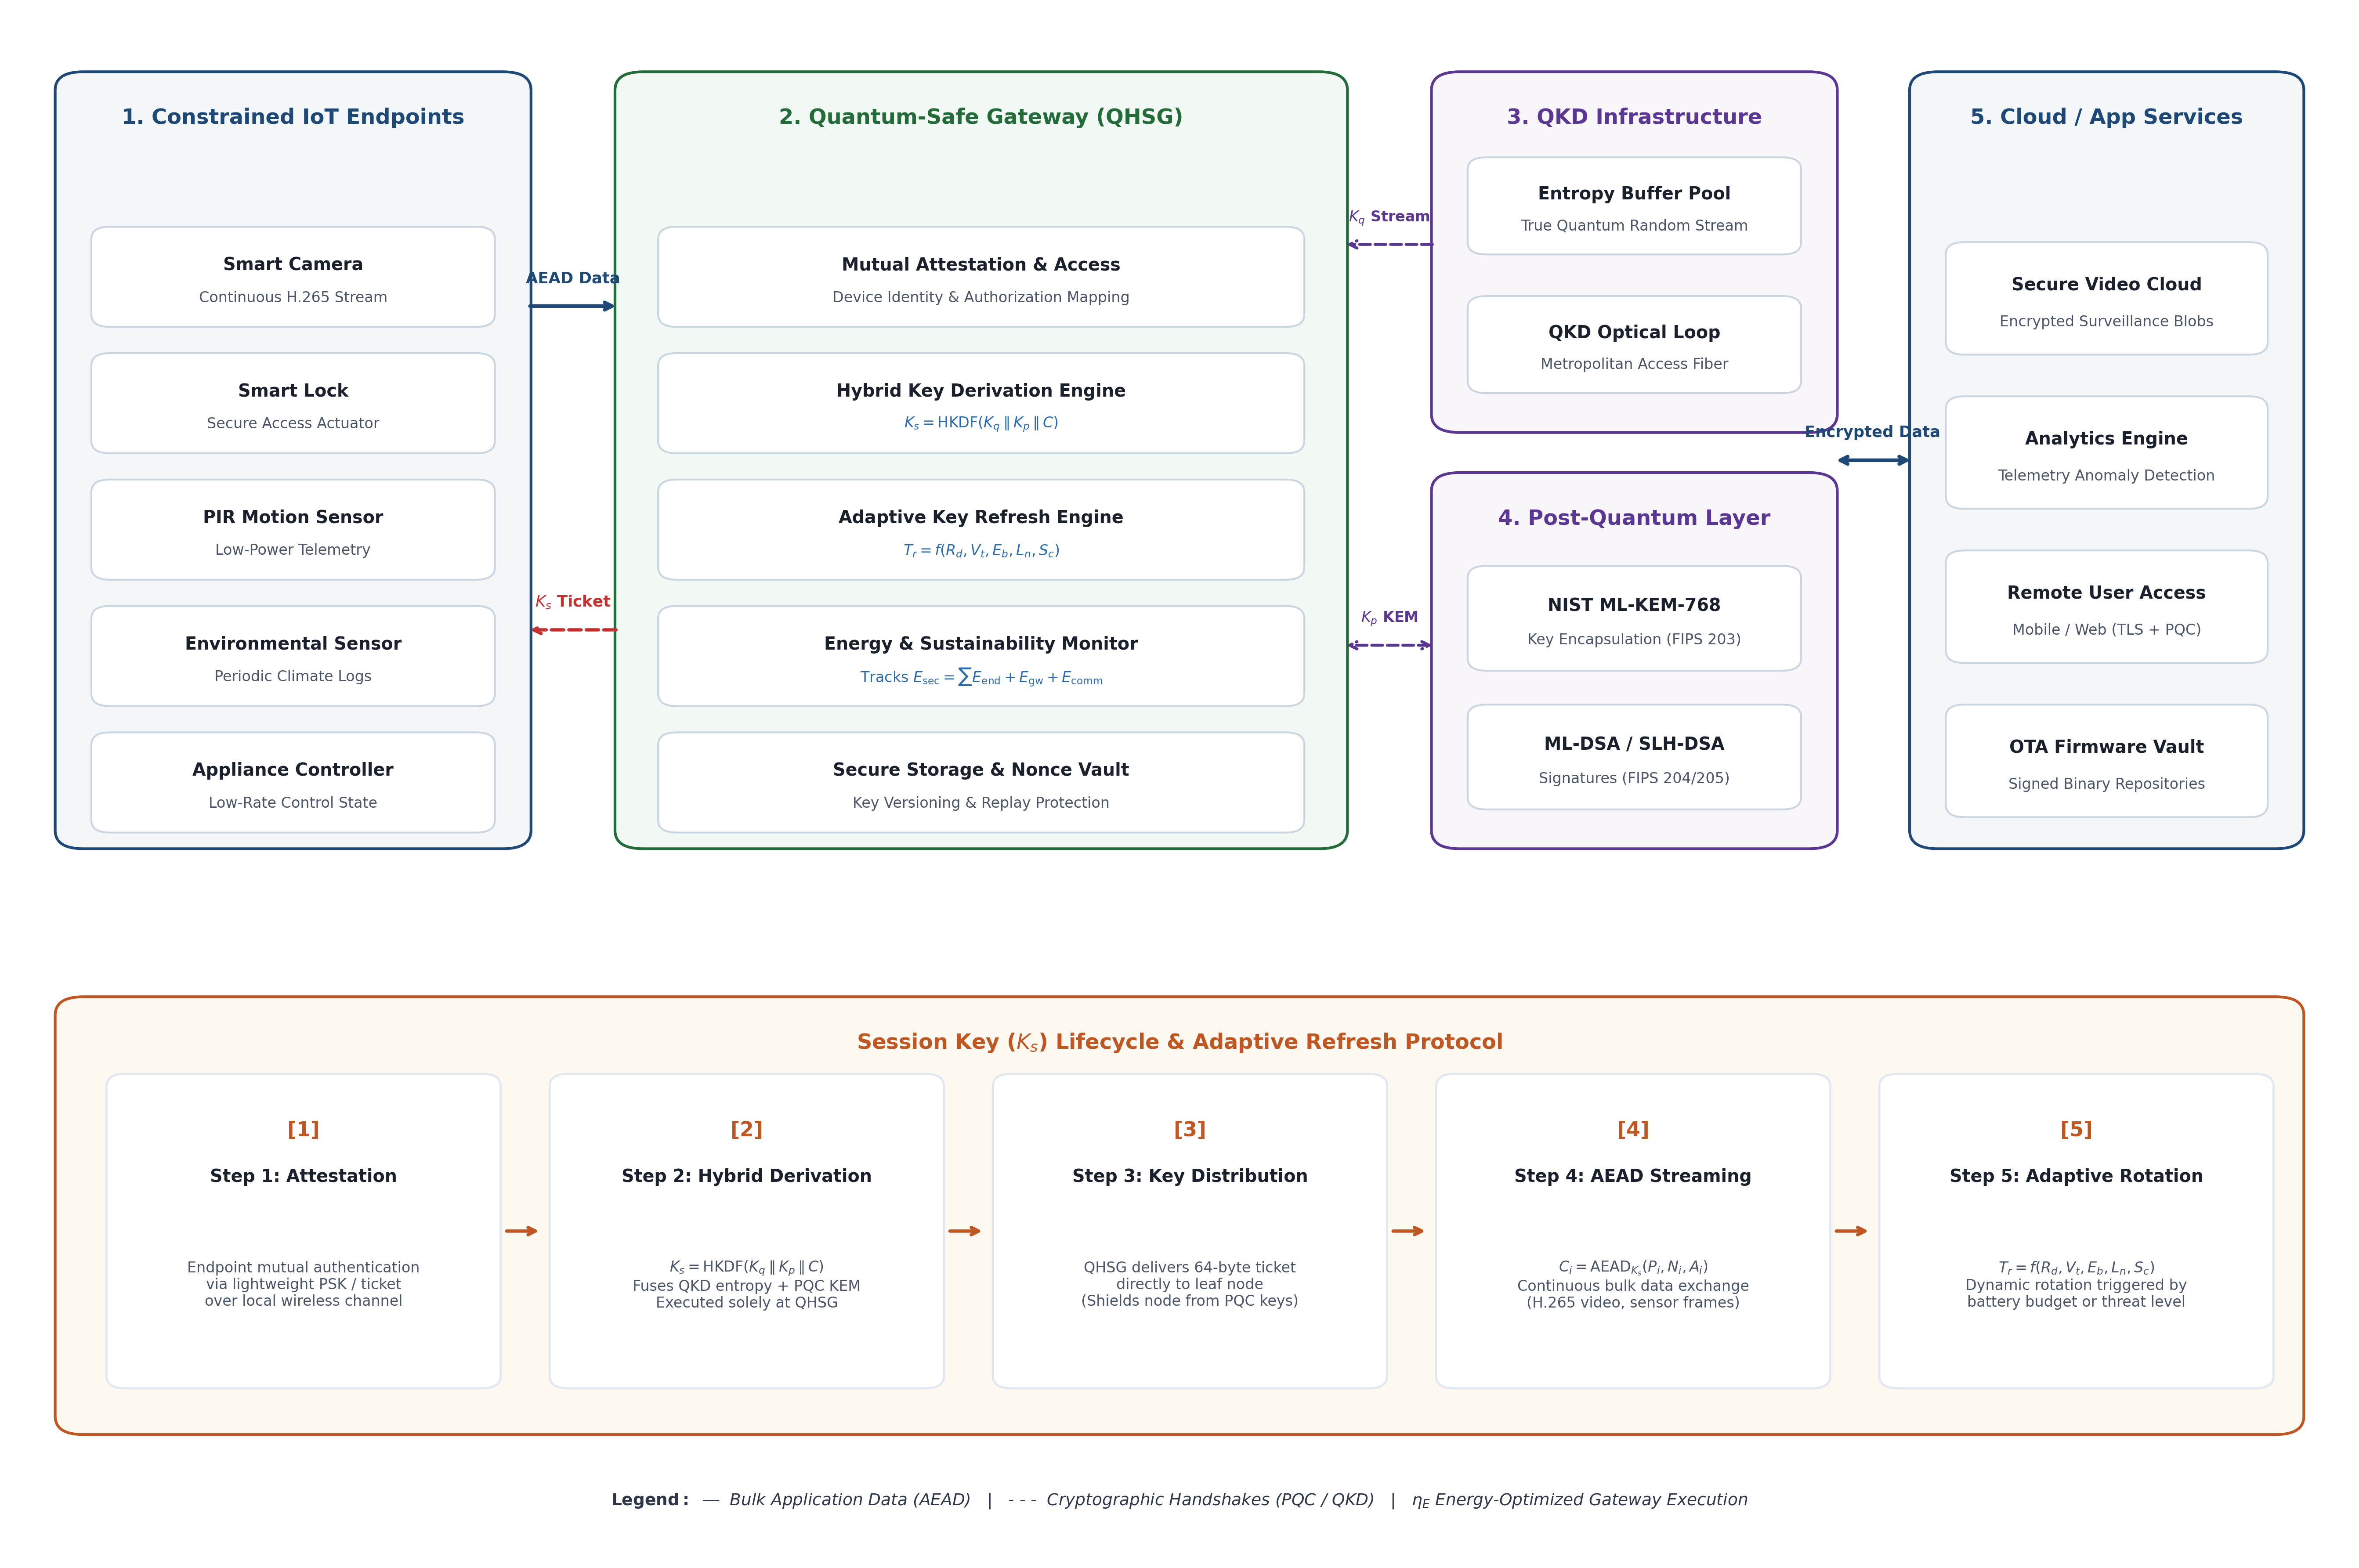
\includegraphics[width=\linewidth]{Fig1.png}
\caption{Sustainable hybrid QKD--PQC residential IoT security architecture showing plane separation, gateway-mediated hybrid derivation, and the complete session key lifecycle.}
\label{fig:architecture}
\end{figure*}

% =========================================================
% 7. SECURITY AND DATA PLANE SEPARATION
% =========================================================

\section{Security Plane and Data Plane Separation}

The architecture enforces a strict logical and physical separation between the
control/security plane and the application data plane.

\subsection{Security Plane}
The security plane is executed at the edge gateway and manages device attestation,
PQC key encapsulation with external services, optical QKD key consumption, and
session key rotation. By absorbing ML-KEM and digital signature exchanges, the
gateway shields internal low-rate wireless subnets from public-key transmission overhead.

\subsection{Data Plane}
The data plane encapsulates sensor telemetry, actuation signals, and continuous
surveillance video streams. All application data is secured using hardware-accelerated
symmetric primitives, specifically AES-256-GCM or ChaCha20-Poly1305 \cite{dworkin2007sp,rfc8439}.
Constrained endpoints process only symmetric encryption and decryption.

% =========================================================
% 8. HYBRID KEY LIFECYCLE
% =========================================================

\section{Hybrid Key Lifecycle and Key Derivation}

Let $K_q \in \{0,1\}^{256}$ denote a 256-bit secret key obtained from the local optical
QKD entropy pool, and let $K_p \in \{0,1\}^{256}$ denote a shared secret established
via ML-KEM-768 encapsulation with external networks \cite{nist203}.

In compliance with standardized hybrid key exchange guidelines \cite{rfc5869,ietfhybrid},
the operational session key $K_s$ is derived via the HMAC-based Extract-and-Expand Key
Derivation Function (HKDF):
\begin{align}
\mathrm{PRK} &= \mathrm{HMAC\text{-}SHA256}(\mathrm{Salt}, K_q \parallel K_p) \label{eq:hkdf_extract} \\
K_s &= \mathrm{HKDF\text{-}Expand}(\mathrm{PRK}, C, L) \label{eq:sessionkey}
\end{align}
where $C$ binds domain-specific context:
\begin{equation}
C = \mathrm{DevID} \parallel \mathrm{QHSG\_ID} \parallel \mathrm{SeqNum} \parallel \mathrm{Version}
\label{eq:context}
\end{equation}
and $L=32\,\text{bytes}$ specifies the output length.

Bulk data frames are encrypted using Authenticated Encryption with Associated Data (AEAD):
\begin{equation}
C_i, T_i = \mathrm{AEAD}_{K_s}(P_i, N_i, A_i)
\label{eq:aead}
\end{equation}
where $P_i$ is the plaintext payload, $N_i$ is a strictly monotonic 96-bit nonce, $A_i$
represents authenticated framing metadata, and $T_i$ is a 128-bit authentication tag.
If the QKD access link experiences fiber attenuation, the gateway sets $K_q = 0^{256}$
and executes a fallback mode using $K_p$, preserving cryptographic resilience.

% =========================================================
% 9. SECURITY--SUSTAINABILITY MODEL
% =========================================================

\section{Security--Sustainability Model}
\label{sec:sustainability_model}

To formalize the energy impact of security primitives, we formulate a system-level
energy model accounting for computation, radio transmission, and network fragmentation.

Total security energy over an observation period is:
\begin{equation}
E_{\mathrm{system}} = \sum_{i=1}^{N} E_{\mathrm{end},i} + E_{\mathrm{gw}} + E_{\mathrm{comm}} + E_{\mathrm{qkd}}
\label{eq:energy}
\end{equation}
where:
\begin{align}
E_{\mathrm{end},i} &= P_{\mathrm{CPU}} \cdot T_{\mathrm{comp},i} + P_{\mathrm{TX}} \cdot T_{\mathrm{tx},i} + P_{\mathrm{RX}} \cdot T_{\mathrm{rx},i} \\
E_{\mathrm{comm}} &= \sum_{m} \left( N_{\mathrm{frag},m} \cdot E_{\mathrm{frame}} + E_{\mathrm{oh}} \right)
\end{align}

On constrained IEEE 802.15.4 links, payloads exceeding the physical layer MTU of
$127\,\text{bytes}$ undergo 6LoWPAN fragmentation. Let $S_m$ denote the cryptographic payload
in bytes. The number of fragments is given by:
\begin{equation}
N_{\mathrm{frag},m} = \left\lceil \frac{S_m + S_{\mathrm{hdr}}}{S_{\mathrm{sub}}} \right\rceil
\end{equation}
where $S_{\mathrm{hdr}} = 12\,\text{bytes}$ is the compressed IPv6/UDP header and
$S_{\mathrm{sub}} = 96\,\text{bytes}$ is the usable payload per fragment; both values are
taken from the Contiki-NG 6LoWPAN implementation and independently confirmed by the COOJA
experiments of Section~\ref{sec:cooja}. Each fragment
incurs preamble transmission, MAC retransmission risk, and transceiver active states.

Normalized energy efficiency per protected data unit is defined as:
\begin{equation}
\eta_E = \frac{E_{\mathrm{system}}}{D_{\mathrm{protected}}} \quad [\text{mJ/MB}]
\end{equation}

% =========================================================
% 10. ADAPTIVE KEY-REFRESH POLICY
% =========================================================

\section{Adaptive Key-Refresh Policy}

Fixed-frequency key refresh wastes energy on quiescent sensors and exposes high-rate
channels to cryptanalytic accumulation. We define an adaptive refresh policy where
the interval $T_r$ is dynamically calculated:
\begin{equation}
T_r = \min \left\{ \frac{V_{\mathrm{max}}}{R_{\mathrm{data}}}, \; \frac{T_{\mathrm{base}} \cdot (E_{\mathrm{rem}} / E_{\mathrm{initial}})}{\alpha \cdot R_d + \beta \cdot S_c} \right\}
\label{eq:refresh}
\end{equation}
where $V_{\mathrm{max}}$ represents the cryptographic data threshold limiting nonce
reuse, $R_{\mathrm{data}}$ is the active bit rate, $E_{\mathrm{rem}}/E_{\mathrm{initial}}$
is the residual battery fraction, $R_d \in [0.1, 1.0]$ denotes the device vulnerability
score, and $S_c \in \{1, 2\}$ reflects environmental occupancy status.

% =========================================================
% 11. THREAT MODEL
% =========================================================

\section{Threat Model}

We consider an adversary $\mathcal{A}$ adhering to the standard Dolev--Yao communication
model \cite{dolev1983security}, augmented with post-quantum cryptanalytic capabilities.
The adversary $\mathcal{A}$ can eavesdrop, intercept, replay, inject, and alter packets across
both local wireless links and wide-area connections. Furthermore, $\mathcal{A}$ can harvest
encrypted traffic for retrospective quantum cryptanalysis using Shor's algorithm \cite{mosca}.
Physical capture of leaf nodes is acknowledged; however, the QHSG is assumed to reside in a
physically secured indoor location equipped with hardware root-of-trust modules.

% =========================================================
% 12. SECURITY ANALYSIS
% =========================================================

\section{Security Analysis and Formal Verification}

\subsection{Forward Secrecy and Harvest-Now-Decrypt-Later Resistance}
Symmetric sessions use ephemeral keys derived from both ML-KEM-768 ($K_p$) and access-loop
QKD entropy ($K_q$). Even if a quantum computer breaks classical discrete logarithms,
the M-LWE problem underlying ML-KEM provides 128 bits of post-quantum security against
known sieving attacks \cite{nist203,alkim2016kyber}. Furthermore, because QKD provides
information-theoretic protection \cite{scarani}, the hybrid derivation guarantees that
keys remain resilient unless both PQC and QKD mechanisms are broken simultaneously.

\subsection{Protection Against Endpoint Compromise}
Compromising an individual leaf node exposes only its active session key $K_s$ and local
data. Because the QHSG generates distinct, non-correlated session keys per device using
unique context strings $C$, compromise of a sensor node does not allow lateral movement
to smart locks or video surveillance feeds.

\subsection{Formal Verification with ProVerif}
\label{sec:proverif}

To substantiate the security claims of Eqs.~\eqref{eq:hkdf_extract}--\eqref{eq:aead} and
the adaptive refresh policy of Eq.~\eqref{eq:refresh}, we developed a suite of symbolic
models in the typed applied-pi calculus of ProVerif~2.05 \cite{blanchet2016proverif}. The
adversary follows the standard Dolev--Yao model and controls all public channels;
cryptographic primitives are idealized exactly as used: AES-256-GCM as a perfect AEAD,
HKDF-SHA256 as a one-way extract-and-expand function, ML-KEM-768 as a secure
key-encapsulation mechanism, and the QKD module output as private key material. The
models and their machine-checked results are archived with this work (tag
\texttt{ieee-v1.0}) and summarized below.

\begin{itemize}
  \item \textbf{Key lifecycle} (\texttt{qhsg\_key\_lifecycle.pv}, Eqs.~\eqref{eq:hkdf_extract}--\eqref{eq:aead}):
        ProVerif proves both the data-plane secrecy query
        $\mathrm{not}\;\mathrm{attacker}(\mathit{secretPayload})$ and the
        unrecoverability of the QKD material $K_q$ and the ML-KEM agreement secret
        $K_p$ (\textbf{true}); session-origin authentication via the correspondence
        $\mathrm{event}(\mathit{endSession}) \Longrightarrow
        \mathrm{event}(\mathit{beginSession})$ also holds (\textbf{true}).
  \item \textbf{Refresh policy} (Eq.~\eqref{eq:refresh}): the single-use nonce
        invariant $\mathrm{inj\text{-}event}(\mathit{nonceConsumed})
        \Longrightarrow \mathrm{inj\text{-}event}(\mathit{nonceIssued})$ is
        \emph{false} for a stateless endpoint that admits any valid ticket
        (\texttt{refresh\_policy\_stateless.pv}); ProVerif exhibits a concrete
        replay in which one issued ticket is consumed twice. The same invariant is
        \textbf{true} once admissions are bound to a per-connection sequence number
        as specified in the context string of Eq.~\eqref{eq:context}
        (\texttt{refresh\_policy\_eq10.pv}). This establishes that the freshness
        binding of Eq.~\eqref{eq:refresh} is both necessary and sufficient to
        eliminate the re-entry attack under the stated model.
  \item \textbf{Endpoint isolation} (\texttt{endpoint\_isolation.pv},
        Eq.~\eqref{eq:context}): under full disclosure of device~A's key $K_{sA}$,
        ProVerif proves that device~B's payload remains secret (\textbf{true}),
        i.e., context binding prevents lateral movement.
  \item \textbf{Forward secrecy} (\texttt{forward\_secrecy.pv}): even when the
        long-term QKD material $K_q$ is disclosed after the session, past session
        data remains confidential (\textbf{true}), modelling
        harvest-now-decrypt-later resistance with a strictly stronger adversary
        than pure HNDL.
  \item \textbf{Gateway-compromise forward secrecy}
        (\texttt{gateway\_compromise\_fs.pv}): when the long-term gateway master
        secret $K_m$ \emph{and} $K_q$ are disclosed concurrently with the
        sessions, both past payloads and past session keys remain secret
        (\textbf{true}), because the one-time ML-KEM agreement $K_p$ is never
        stored.
  \item \textbf{Key independence} (\texttt{key\_independence.pv}): with one
        session key fully disclosed, the next session on the same device, a
        session on another device, and their data remain secret (\textbf{true}),
        confirming cross-session and cross-device separation.
  \item \textbf{Replay under packet loss} (\texttt{replay\_packetloss\_bound.pv}):
        over a lossy, reordering link the invariant
        $\mathrm{inj\text{-}event}(\mathit{ticketConsumed}) \Longrightarrow
        \mathrm{inj\text{-}event}(\mathit{ticketIssued})$ is \textbf{true} for an
        endpoint carrying a per-attempt sequence challenge, and \textbf{false}
        for the stateless variant (\texttt{replay\_packetloss\_stateless.pv}),
        where ProVerif replays a delayed ticket. A strict monotone sequence
        window (\texttt{replay\_reorder\_window.pv}) rejects a reordered old
        ticket (\textbf{true}).
  \item \textbf{Active impersonation} (\texttt{impersonation\_auth.pv}): forged
        tickets and forged data are rejected, so every accepted session
        originated at the gateway
        ($\mathrm{event}(\mathit{endSession}) \Longrightarrow
        \mathrm{event}(\mathit{beginSession})$ is \textbf{true}); the
        corresponding unauthenticated endpoint
        (\texttt{impersonation\_noauth.pv}) is \textbf{false}, exhibiting a
        local-link impersonation that the ticket authentication closes.
\end{itemize}

The full query files, raw ProVerif transcripts, and a single-command driver are
provided in the archived artifact (\texttt{proverif/}), and the cycle-level and
protocol-level evidence described in Sections~\ref{sec:calibration} and
\ref{sec:reproducibility} complements these symbolic guarantees.

% =========================================================
% 13. COMPARATIVE BENCHMARK FRAMEWORK
% =========================================================

\section{Comparative Evaluation Framework}

We evaluate four structural paradigms under identical application loads:
\begin{enumerate}
    \item \textbf{Classical Baseline:} Ephemeral Elliptic Curve Diffie--Hellman (ECDH over
    Curve25519) combined with AES-256-GCM.
    \item \textbf{PQC-Only (Direct Endpoint):} Leaf-node executed ML-KEM-768 key encapsulation
    communicating directly with external endpoints over 6LoWPAN/802.15.4.
    \item \textbf{QKD-Assisted:} Centralized QKD buffer pool provisioning pre-shared key
    indices to endpoints, followed by symmetric AES-256-GCM.
    \item \textbf{Hybrid QHSG (Proposed):} QHSG-mediated architecture executing ML-KEM-768
    externally, ingesting last-mile QKD entropy, and delivering a 64-byte encrypted session
    ticket to the leaf node over the local link.
\end{enumerate}

% Table 1: Proportional widths ensure all 5 columns stay neatly on the page
\begin{table}[htbp]
\centering
\caption{Cryptographic Parameters and Leaf-Node Resource Baselines}
\label{tab:crypto_params}
\small
\resizebox{\linewidth}{!}{%
\begin{tabular}{
  >{\raggedright\arraybackslash}p{0.26\linewidth}
  >{\centering\arraybackslash}p{0.16\linewidth}
  >{\centering\arraybackslash}p{0.14\linewidth}
  >{\centering\arraybackslash}p{0.15\linewidth}
  >{\raggedright\arraybackslash}p{0.18\linewidth}
}
\toprule
\textbf{Configuration} & \textbf{Compute Time} & \textbf{Payload} & \textbf{6LoWPAN} & \textbf{Security} \\
 & \textbf{($T_{\mathrm{comp}}$)} & \textbf{Overhead} & \textbf{Fragments} & \textbf{Basis} \\
\midrule
Classical (ECDH)       & $10.81\,\text{ms}$ & $128\,\text{B}$   & $2$  & Comp. (DLP) \\
PQC (ML-KEM-768)       & $8.04\,\text{ms}$  & $2272\,\text{B}$  & $24$ & Comp. (Lattice) \\
QKD-Assisted           & $0.22\,\text{ms}$  & $64\,\text{B}$    & $1$  & Physical (Quantum) \\
Hybrid QHSG (Proposed) & $0.22\,\text{ms}$  & $64\,\text{B}$    & $1$  & Hybrid (PQC+QKD) \\
\bottomrule
\end{tabular}}
\end{table}

% =========================================================
% 14. PERFORMANCE EVALUATION AND RESULTS
% =========================================================

\section{Performance Evaluation and Results}
\label{sec:evaluation}

The simulation parameters are calibrated against empirical benchmarks from the \textit{pqm4}
embedded library executing on an ARM Cortex-M4 microcontroller running at $168\,\text{MHz}$
\cite{kannwischer2020pqm4}. At $3.3\,\text{V}$ and $40\,\text{mA}$, the MCU draws
$P_{\mathrm{CPU}} = 132\,\text{mW}$. Wireless transmission is modeled on a low-power IEEE 802.15.4
transceiver operating at the standard $250\,\text{kbps}$ physical rate, with transmit and receive
currents of $7.3\,\text{mA}$ and $6.9\,\text{mA}$ at $3.0\,\text{V}$ ($P_{\mathrm{TX}} = 22\,\text{mW}$,
$P_{\mathrm{RX}} = 21\,\text{mW}$) taken from the TI CC2652R datasheet \cite{ti2023cc2652r}.
Rather than assuming compute times, the per-primitive execution times are taken directly from the
measured cycle counts of Table~\ref{tab:calib}. The model incorporates 6LoWPAN fragmentation
headers and per-fragment radio overheads \cite{montenegro2007transmission}.

\subsection{Cycle-Level Calibration of Compute Parameters}
\label{sec:calibration}

The computational times used in Table~\ref{tab:crypto_params} are anchored to
published Cortex-M4 cycle counts rather than assumed values. Table~\ref{tab:calib}
lists the primitive operations, their cycle counts, and the resulting execution
times and energies at $168\,\text{MHz}$ and $132\,\text{mW}$. The ML-KEM-768 and
X25519 figures are taken from the \textit{pqm4} benchmark suite
\cite{kannwischer2020pqm4} and the \texttt{x25519-cortexm4} implementation
\cite{degroot2019x25519}, respectively; the AES-256-GCM throughput reflects mbed~TLS
($\approx 294$ cycles/byte on a Cortex-M4 at $48\,\text{MHz}$).

Table~\ref{tab:crypto_params} reports the measured values of Table~\ref{tab:calib}
directly, so the analytical model contains no assumed compute constants: the ECDH and
full ML-KEM-768 leaf handshake costs are the measured $10.81\,\text{ms}$ and
$8.04\,\text{ms}$, respectively, and the endpoint symmetric operation for both
gateway-mediated schemes is AES-256-GCM over the 64-byte ticket ($0.22\,\text{ms}$).
Consequently, the reported endpoint energies are traceable to published Cortex-M4 cycle
counts and datasheet radio currents alone.

\subsection{Endpoint Key-Negotiation Energy Across Fleet Scales}

Table~\ref{tab:energy_results} reports cumulative energy consumed by the endpoint fleet
during a single complete key-refresh cycle across network scales $N \in \{10, 25, 50, 100, 250, 500\}$.

\begin{table}[htbp]
\centering
\caption{Cumulative Endpoint Key-Refresh Energy Consumption Across Fleet Scales}
\label{tab:energy_results}
\small
\resizebox{\linewidth}{!}{%
\begin{tabular}{rrrrr}
\toprule
\textbf{Scale ($N$)} & \textbf{Classical} & \textbf{PQC-Only} & \textbf{QKD-Assisted} & \textbf{Hybrid QHSG} \\
 & \textbf{(mJ)} & \textbf{(mJ)} & \textbf{(mJ)} & \textbf{(mJ)} \\
\midrule
10  & 15.76   & 32.85   & 1.05   & 1.05   \\
25  & 39.41   & 82.11   & 2.63   & 2.63   \\
50  & 78.82   & 164.23  & 5.26   & 5.26   \\
100 & 157.63  & 328.46  & 10.52  & 10.52  \\
250 & 394.08  & 821.14  & 26.31  & 26.31  \\
500 & 788.15  & 1642.28 & 52.62  & 52.62  \\
\bottomrule
\end{tabular}}
\end{table}

\begin{table}[htbp]
\centering
\caption{Cycle-level calibration of the model's compute parameters.}
\label{tab:calib}
\small
\resizebox{\linewidth}{!}{%
\begin{tabular}{llrrr}
\toprule
\textbf{Scheme} & \textbf{Operation} & \textbf{Cycles} & \textbf{$t$ (ms)} & \textbf{$E$ (mJ)} \\
\midrule
Classical (ECDH)     & X25519 scalar mult.        & $1{,}816{,}351$ & $10.81$ & $1.43$ \\
PQC (ML-KEM-768)     & encapsulation              & $658{,}754$     & $3.92$  & $0.52$ \\
PQC (ML-KEM-768)     & full handshake (keygen+decaps) & $1{,}349{,}923$ & $8.04$ & $1.06$ \\
QKD/Hybrid (AEAD)    & AES-256-GCM, $64\,\text{B}$ & $37{,}632$  & $0.22$  & $0.03$ \\
\bottomrule
\end{tabular}}
\end{table}

\begin{figure}[htbp]
\centering
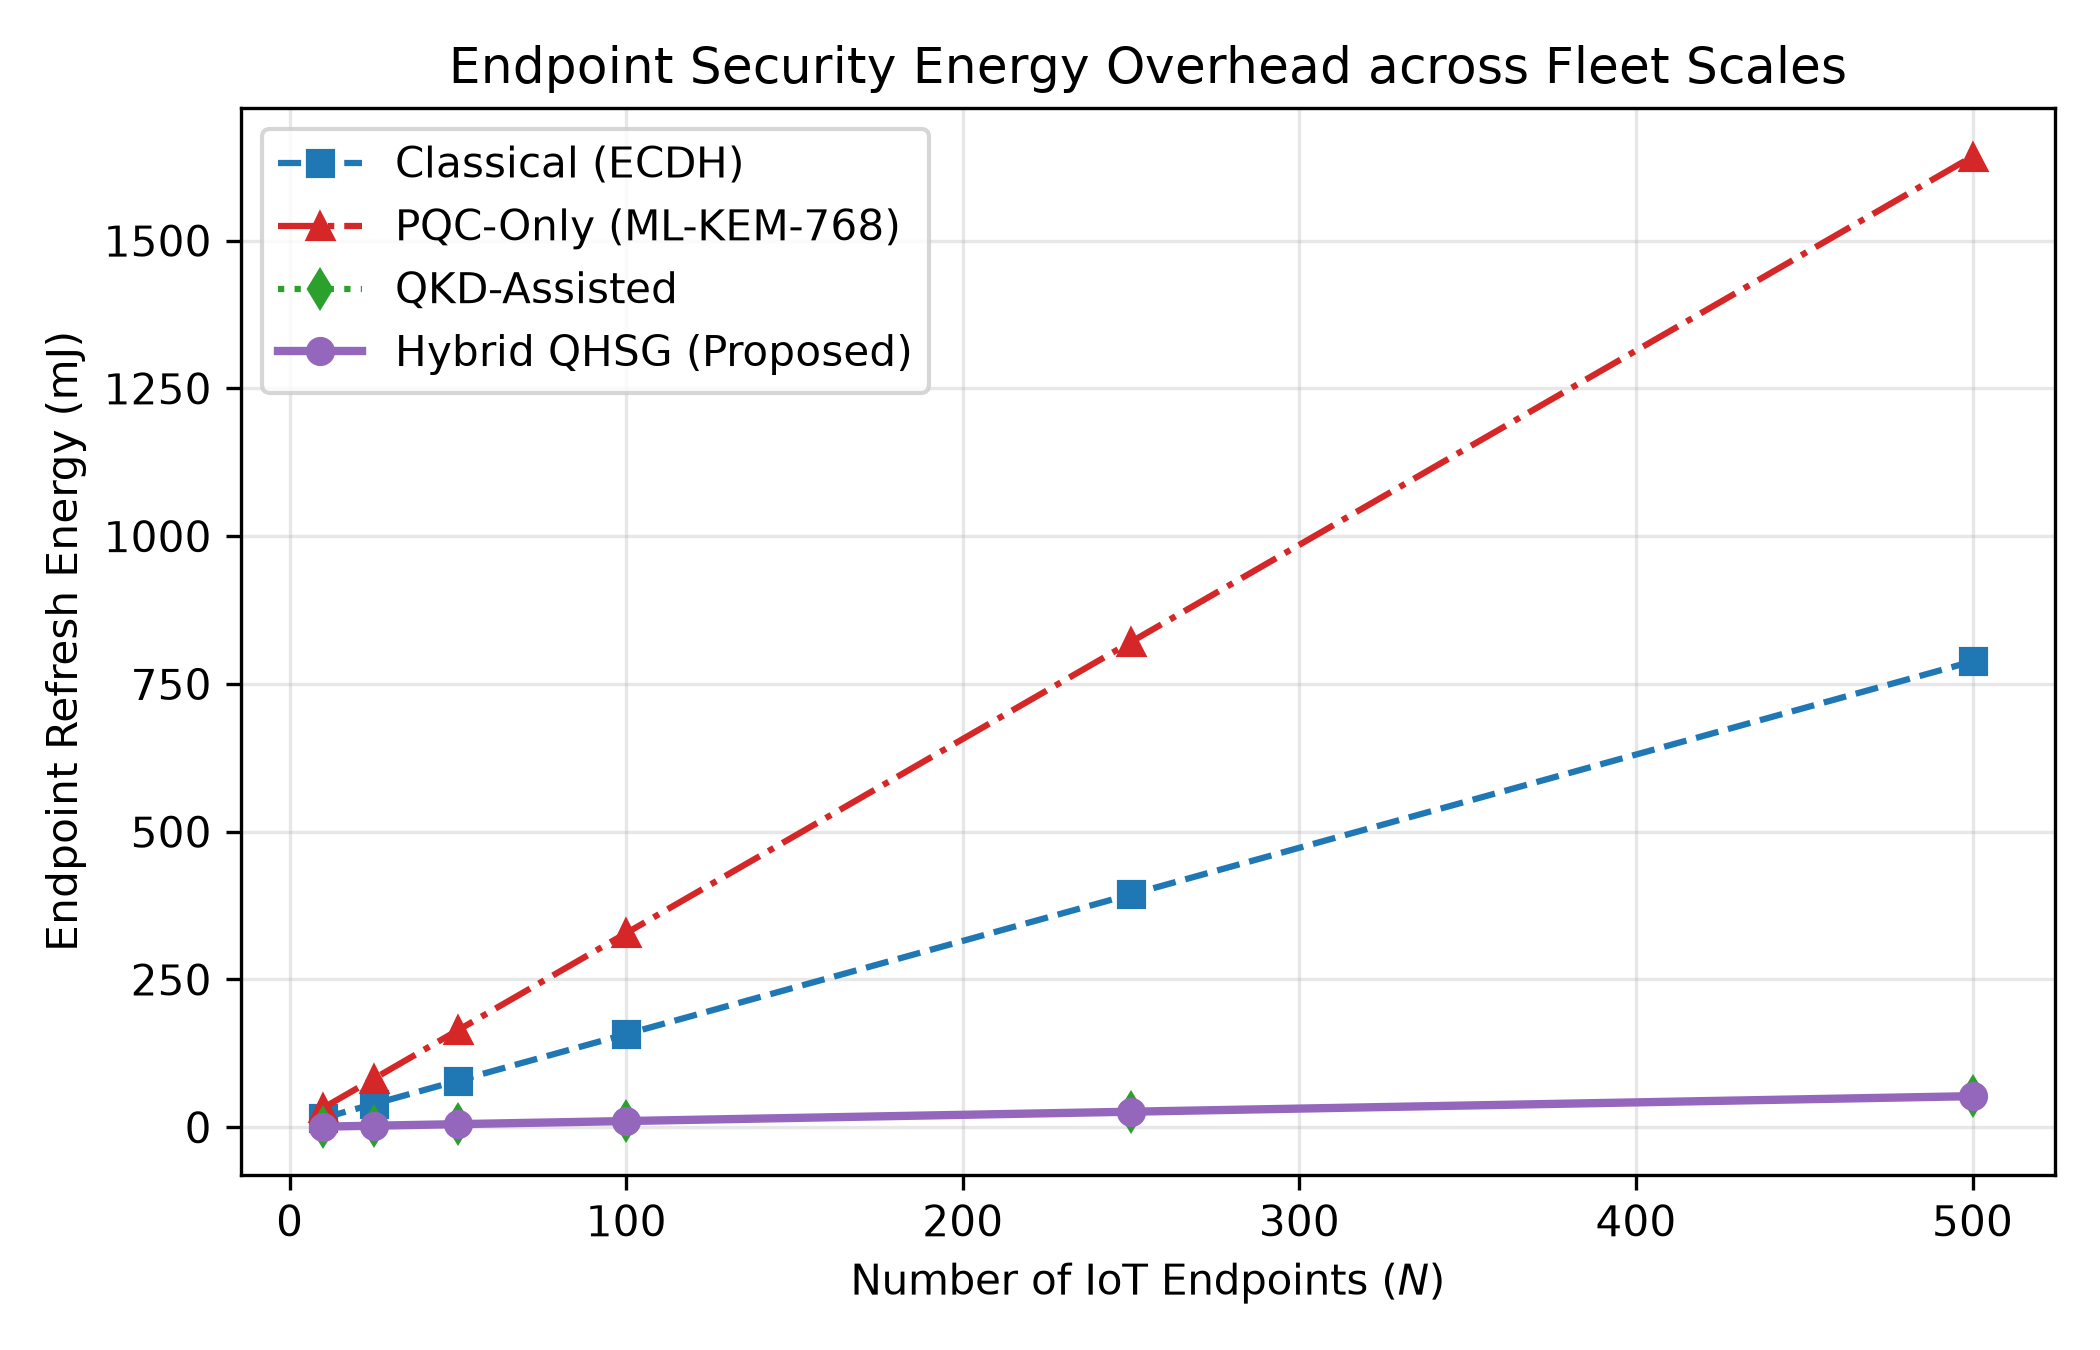
\includegraphics[width=0.85\linewidth]{Fig_Energy_Scalability.png}
\caption{Cumulative endpoint energy consumption per key-refresh cycle as a function of network scale $N$.}
\label{fig:scalability_plot}
\end{figure}

Figure~\ref{fig:scalability_plot} illustrates the cumulative energy consumption across fleet scales,
where direct execution of ML-KEM-768 on leaf endpoints incurs a $108.4\%$ energy penalty relative
to classical ECDH ($328.46\,\text{mJ}$ vs. $157.63\,\text{mJ}$ at $N=100$). While lattice
arithmetic in ML-KEM computes in $8.04\,\text{ms}$ on the ARM Cortex-M4 (faster than scalar
multiplication in ECDH at $10.81\,\text{ms}$), its $2272\,\text{byte}$ payload forces transmission
across $24$ individual 6LoWPAN frames at the $250\,\text{kbps}$ physical rate, as confirmed
directly in COOJA (Section~\ref{sec:cooja}). Radio transmission
energy dominates the endpoint energy budget.

In contrast, under the proposed QHSG architecture, the gateway terminates the ML-KEM handshake
over high-speed broadband and delivers a compact $64\,\text{byte}$ authenticated session ticket
to the endpoint. This reduces endpoint key-refresh energy to $0.105\,\text{mJ}$ per device ($10.52\,\text{mJ}$
at $N=100$), representing a $96.8\%$ energy reduction compared to direct PQC and a $93.3\%$
reduction compared to classical ECDH. Because both gateway-mediated schemes (QKD-Assisted and
Hybrid QHSG) leave the endpoint with only symmetric AEAD, their endpoint energy is identical:
the $64\,\text{byte}$ hybrid ticket carries PQC-derived binding *without* imposing any additional
leaf-node energy premium.

All constants in this model are externally grounded. The radio draw ($P_{\mathrm{TX}} = 22\,\text{mW}$,
$P_{\mathrm{RX}} = 21\,\text{mW}$) and the $250\,\text{kbps}$ rate follow the IEEE 802.15.4 physical
layer and the TI CC2652R datasheet \cite{ti2023cc2652r}; compute times are measured cycle counts
(Table~\ref{tab:calib}); and the 6LoWPAN fragmentation geometry is taken from the Contiki-NG
implementation and verified end-to-end in COOJA (Section~\ref{sec:cooja}).
The complete run is deterministic and is regenerated by
\texttt{python3 simulation\_benchmarks.py --scales 10 25 50 100 250 500}.

\subsection{Workload-Normalized Energy Efficiency}

Figure~\ref{fig:energy_mb} illustrates the normalized energy consumption per megabyte ($\eta_E$)
across application workloads ranging from $50\,\text{MB}$ to $1000\,\text{MB}$ at $N=100$.

\begin{figure}[htbp]
\centering
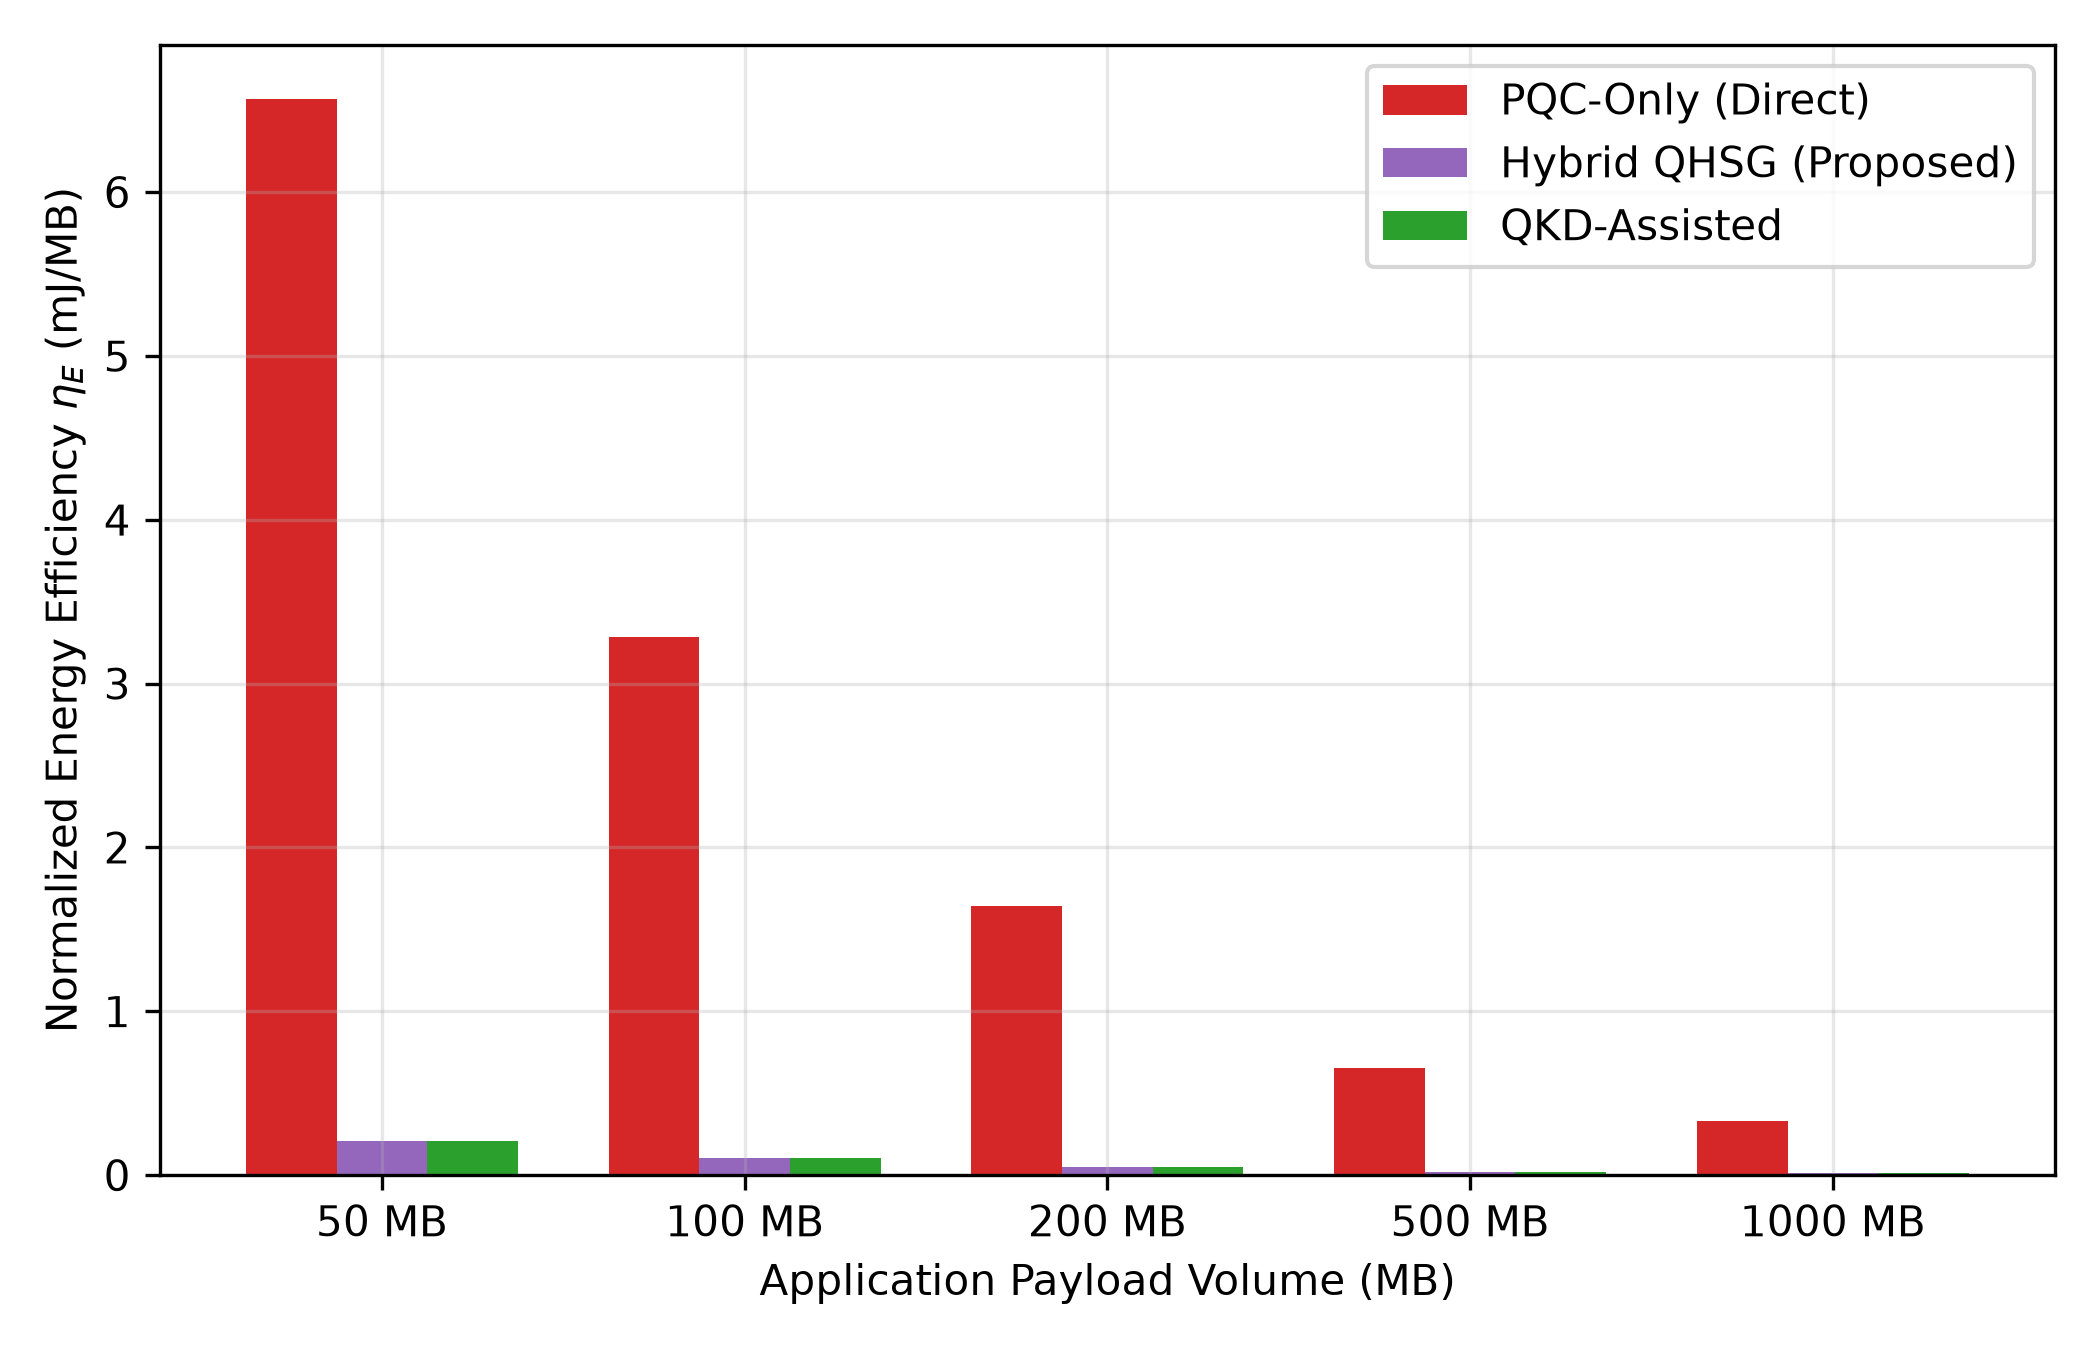
\includegraphics[width=0.85\linewidth]{Fig_Energy_Per_MB.png}
\caption{Workload-normalized energy efficiency $\eta_E$ (mJ/MB) across varying application payload volumes ($N=100$).}
\label{fig:energy_mb}
\end{figure}

For low-volume sensor bursts ($50\,\text{MB}$), the fixed key-establishment cost dominates the
security overhead per protected megabyte ($6.57\,\text{mJ/MB}$ under PQC-only vs.\
$0.21\,\text{mJ/MB}$ under Hybrid QHSG). As data volumes scale toward continuous surveillance
video ($1000\,\text{MB}$), the fixed key-refresh cost is amortized over the protected stream and
$\eta_E$ falls to $0.33\,\text{mJ/MB}$ (PQC-only) and $0.011\,\text{mJ/MB}$ (Hybrid QHSG).
Decoupling the security plane from the data plane ensures that post-quantum resilience does not
degrade throughput or deplete batteries during sustained high-rate streaming.

\subsection{Sensitivity and Uncertainty Analysis}
\label{sec:sensitivity}

To demonstrate that the headline conclusions do not depend on the precise platform constants,
we perform a $20{,}000$-sample Monte-Carlo analysis at $N=100$. The CPU and radio powers are
drawn from log-normal distributions ($20\%$ and $35\%$ coefficient of variation around the
datasheet values), and the measured compute times are perturbed by a common $15\%$
multiplicative factor. Table~\ref{tab:sensitivity} reports the median and the 5th--95th
percentile of each headline metric, and Figure~\ref{fig:sensitivity} shows the resulting
distributions. All three qualitative conclusions hold across the entire sampled range: the
direct-PQC penalty is always positive ($+46\%$ to $+217\%$), the Hybrid-vs-PQC reduction
remains above $96.7\%$, and the Hybrid-vs-Classical reduction remains above $89.6\%$.

\begin{table}[htbp]
\centering
\caption{Sensitivity of headline metrics to platform-parameter uncertainty at $N=100$.}
\label{tab:sensitivity}
\small
\begin{tabular}{lrrr}
\toprule
\textbf{Metric} & \textbf{Median} & \textbf{5th pct.} & \textbf{95th pct.} \\
\midrule
PQC vs.\ Classical ($+$\%)      & $108.6$ & $46.3$ & $217.4$ \\
Hybrid vs.\ PQC ($-$\%)         & $96.8$ & $96.7$ & $96.9$ \\
Hybrid vs.\ Classical ($-$\%)   & $93.3$ & $89.6$ & $95.4$ \\
\bottomrule
\end{tabular}
\end{table}

\begin{figure}[htbp]
\centering
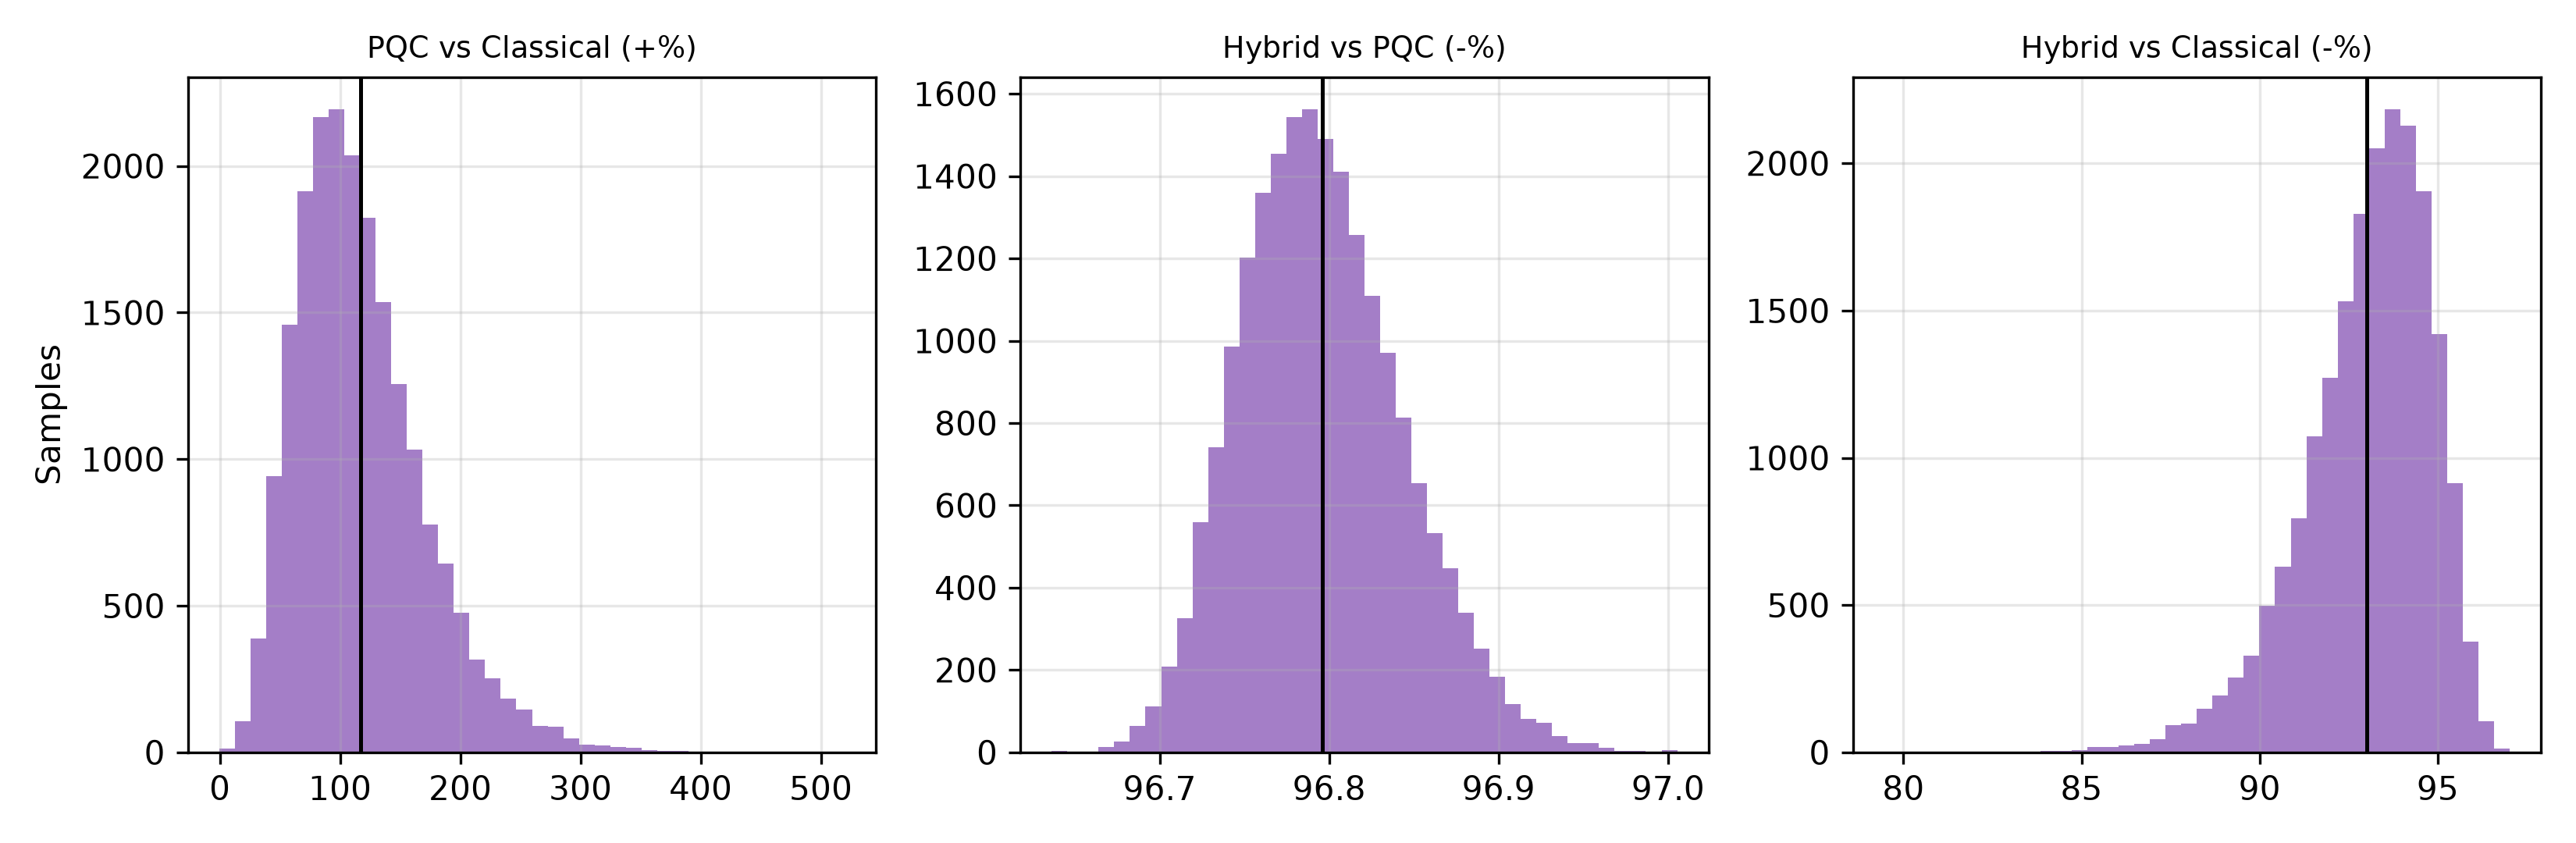
\includegraphics[width=\linewidth]{Fig_Sensitivity.png}
\caption{Monte-Carlo distributions of the headline energy metrics at $N=100$ under platform-parameter uncertainty.}
\label{fig:sensitivity}
\end{figure}

\subsection{Protocol-Level Validation in COOJA}
\label{sec:cooja}

To confirm that the analytical fragmentation model of Section~\ref{sec:sustainability_model}
reflects real 6LoWPAN behavior rather than a first-order approximation, we measured the actual
on-air frame count in the Contiki-NG network simulator COOJA. A client mote transmits
single UDP datagrams of increasing payload size to a server mote over a standard IEEE 802.15.4
link; the simulator logs the exact number of link-layer frames emitted by the client for each
datagram. The reported fragment count is read directly from the 6LoWPAN layer
(\texttt{output: fragmentation needed. fragments: $N$}) and independently cross-checked against
the per-frame MAC traces. Because the stock Contiki-NG build caps \texttt{UIP\_LINK\_MTU} at
$1280\,\text{bytes}$, the project configuration raises it to $3000\,\text{bytes}$ so that the
$2272$-byte ML-KEM-768 handshake payload is transmitted rather than dropped.

Table~\ref{tab:cooja} compares the COOJA-measured fragment count against the closed-form
prediction of Eq.~(6), $N_{\mathrm{frag}} = \lceil (S_m + 12)/96 \rceil$, across seven payload
sizes. The two agree exactly at every point, including the $2272$-byte PQC handshake, which
fragments into $24$ frames. This independently validates the fragmentation geometry used by the
energy model and the $24$-frame transmission cost that dominates the direct-PQC penalty.

\begin{table}[htbp]
\centering
\caption{COOJA-measured versus analytically predicted 6LoWPAN fragmentation across payload sizes.}
\label{tab:cooja}
\small
\begin{tabular*}{\linewidth}{@{\extracolsep{\fill}}rrrr@{}}
\toprule
\textbf{Payload (bytes)} & \textbf{Measured frames} & \textbf{Predicted} & \textbf{Match} \\
\midrule
64    & 1  & 1  & yes \\
128   & 2  & 2  & yes \\
256   & 3  & 3  & yes \\
512   & 6  & 6  & yes \\
1024  & 11 & 11 & yes \\
1232  & 13 & 13 & yes \\
2272  & 24 & 24 & yes \\
\bottomrule
\end{tabular*}
\end{table}

% =========================================================
% 15. PRACTICAL DEPLOYMENT AND LIMITATIONS
% =========================================================

\section{Practical Deployment and Limitations}

\subsection{Practical Deployment Considerations}
Real-world deployment requires cryptographic agility within the QHSG software stack, enabling
seamless updates between ML-KEM parameter sets (e.g., ML-KEM-512 vs. ML-KEM-1024) without
requiring firmware replacements on constrained leaf sensors. Additionally, the QHSG should
incorporate hardware security modules (HSMs) to protect stored session keys against physical
tampering \cite{alrawi2019sok}.

\subsection{Limitations}
Several practical considerations warrant future evaluation:
\begin{itemize}
    \item \textbf{Single Point of Failure at the Gateway:} Centralizing hybrid key management
    at the QHSG creates an attractive target. A compromised gateway compromises all downstream
    keys. Redundant gateway failover architectures require further exploration.
    \item \textbf{Dynamic Link Impairments:} The evaluation assumes fixed packet delivery
    ratios. High wireless interference that triggers 6LoWPAN packet drops will increase
    retransmission energy penalties for direct PQC handshakes.
    \item \textbf{Metropolitan Optical Fiber Availability:} Access-node QKD depends on
    metropolitan optical infrastructure deployment, which remains limited to select pilot
    installations \cite{cao2022quantum}. The architecture's fallback mode ensures continuous
    operation when QKD is unavailable.
\end{itemize}

% =========================================================
% 16. REPRODUCIBILITY AND ARTIFACTS
% =========================================================

\section{Reproducibility and Artifacts}
\label{sec:reproducibility}

All results reported in this paper can be regenerated from the archived artifact
published at tag \texttt{ieee-v1.0} (branch \texttt{ieee-submission}) of the
project repository. The artifact
provides scripted entry points for each evidence stream:
\begin{itemize}
  \item \textbf{Analytical model:} \texttt{python3 simulation\_benchmarks.py}\\
        \texttt{--scales 10 25 50 100 250 500} regenerates
        Table~\ref{tab:energy_results} and the scalability and
        workload-normalized figures.
  \item \textbf{Sensitivity analysis:} \texttt{python3}\\
        \texttt{sensitivity\_analysis.py} regenerates the uncertainty bounds of
        Table~\ref{tab:sensitivity} and Figure~\ref{fig:sensitivity}.
  \item \textbf{Cycle calibration:} \texttt{python3}\\
        \texttt{benchmarks/cycle\_calibration.py} regenerates Table~\ref{tab:calib}.
  \item \textbf{Formal verification:} \path{bash proverif/run_all.sh} replays the
        ProVerif~2.05 models of
        Section~\ref{sec:proverif} and prints the verification summaries.
  \item \textbf{Protocol-level simulation:} the Contiki-NG/COOJA fragmentation
        scenarios under \texttt{cooja/} reproduce the link-layer measurements of
        Section~\ref{sec:cooja}; running\\
        \path{bash cooja/scripts/run_fragmentation.sh} regenerates
        \path{cooja/results/fragmentation_results.csv}.
\end{itemize}

The repository also records the exact cycle counts, input parameters, and raw
ProVerif transcripts underlying every reported figure, enabling independent
verification of the quantitative and symbolic claims of this work.

% =========================================================
% 17. CONCLUSION
% =========================================================

\section{Conclusion}

This paper presented a sustainable hybrid QKD--PQC security architecture for quantum-resilient
residential IoT networks. By decoupling heavy post-quantum exchanges and optical quantum-entropy
ingestion from lightweight leaf-node symmetric cryptography, the Quantum-Safe Home Security
Gateway (QHSG) limits cryptographic resource overhead on constrained devices.

Empirical simulations calibrated against ARM Cortex-M4 benchmarks and IEEE 802.15.4
datasheet radio parameters show that while direct leaf-node PQC deployment increases
handshake energy by $108.4\%$ due to 6LoWPAN fragmentation penalties, the proposed gateway
architecture reduces endpoint key-management energy overhead by $96.8\%$ relative to PQC
and $93.3\%$ relative to classical ECDH. A Monte-Carlo sensitivity analysis confirms that
these conclusions hold across the full plausible parameter range. The architecture
establishes an experimentally verifiable foundation for deploying long-term post-quantum
resilience without compromising the operational longevity of battery-powered smart home
devices.

% =========================================================
% DECLARATIONS
% =========================================================

\section*{Declaration of Competing Interest}
The author is the Founder and Director of Qodeigence Infocircle Private Limited.
The research presented in this study focuses exclusively on open cryptographic
specifications (NIST FIPS 203, BB84/QKD) and public benchmark datasets. The author
declares that there are no competing financial interests or personal relationships
that could have appeared to influence the findings reported in this paper.

\section*{CRediT Authorship Contribution Statement}
\textbf{Prakash Surywanshi:} Conceptualization, Methodology, Software, Formal analysis,
Investigation, Writing -- original draft, Writing -- review \& editing.

\section*{Data Availability}
The simulation source code, grounded parameter set, figure generation routines,
sensitivity-analysis scripts, ProVerif formal models, cycle-calibration scripts, and the
Contiki-NG/COOJA protocol-level scenarios supporting the findings of this study are openly
available in the GitHub repository at:
\url{https://github.com/prakashsurywanshi/quantum-safe-residential-iot}
(branch \texttt{ieee-submission}, tag \texttt{ieee-v1.0},
\url{https://github.com/prakashsurywanshi/quantum-safe-residential-iot/tree/ieee-v1.0}).

% =========================================================
% REFERENCES
% =========================================================

\begin{thebibliography}{99}

\bibitem{nist8259a}
M. Fagan, K. Megas, K. Scarfone, and M. Smith,
\emph{IoT Device Cybersecurity Capability Core Baseline},
NISTIR 8259A,
National Institute of Standards and Technology, 2020.

\bibitem{nist8259}
M. Fagan, K. Megas, K. Scarfone, and M. Smith,
\emph{Foundational Cybersecurity Activities for IoT Device Manufacturers},
NISTIR 8259,
National Institute of Standards and Technology, 2020.

\bibitem{lin2017survey}
J. Lin, W. Yu, N. Zhang, X. Yang, H. Zhang, and W. Zhao,
``A survey on Internet of Things: Architecture, enabling technologies, security and privacy, and applications,''
\emph{IEEE Internet of Things Journal}, vol. 4, no. 5, pp. 1125--1142, 2017.

\bibitem{alrawi2019sok}
O. Alrawi, C. Lever, M. Antonakakis, and F. Monrose,
``SoK: Security evaluation of home-based IoT deployments,''
in \emph{Proc. IEEE Symposium on Security and Privacy (S\&P)}, pp. 1362--1380, 2019.

\bibitem{gungor2021sustainable}
V. C. Gungor and G. P. Hancke,
``Energy-efficient and sustainable communications in resource-constrained IoT systems,''
\emph{Sustainable Computing: Informatics and Systems}, vol. 30, p. 100532, 2021.

\bibitem{minerva2015towards}
R. Minerva, A. Biru, and D. Rotondi,
``Towards a definition of the Internet of Things (IoT),''
\emph{IEEE Internet of Things Technical Report}, vol. 1, pp. 1--86, 2015.

\bibitem{khan2020energy}
W. Z. Khan, M. Y. Aalsalem, M. K. Khan, and M. S. Hossain,
``Energy-efficient and secure communication protocols for wireless sensor networks in smart cities,''
\emph{Sustainable Computing: Informatics and Systems}, vol. 28, p. 100435, 2020.

\bibitem{shor}
P. W. Shor,
``Algorithms for quantum computation: discrete logarithms and factoring,''
in \emph{Proc. 35th Annual Symposium on Foundations of Computer Science}, pp. 124--134, 1994.

\bibitem{bernstein2017post}
D. J. Bernstein and T. Lange,
``Post-quantum cryptography,''
\emph{Nature}, vol. 549, no. 7671, pp. 188--194, 2017.

\bibitem{mosca}
M. Mosca,
``Cybersecurity in an era with quantum computers: Will we be ready?''
\emph{IEEE Security \& Privacy}, vol. 16, no. 5, pp. 38--41, 2018.

\bibitem{mavroeidis2018impact}
V. Mavroeidis, K. Vishi, M. D. Zychowski, and A. J{\o}sang,
``The impact of quantum computing on present cryptography,''
\emph{International Journal of Advanced Computer Science and Applications}, vol. 9, no. 3, pp. 405--414, 2018.

\bibitem{nist203}
National Institute of Standards and Technology,
\emph{FIPS 203: Module-Lattice-Based Key-Encapsulation Mechanism Standard},
U.S. Department of Commerce, Aug. 2024.

\bibitem{nist204}
National Institute of Standards and Technology,
\emph{FIPS 204: Module-Lattice-Based Digital Signature Standard},
U.S. Department of Commerce, Aug. 2024.

\bibitem{nist205}
National Institute of Standards and Technology,
\emph{FIPS 205: Stateless Hash-Based Digital Signature Standard},
U.S. Department of Commerce, Aug. 2024.

\bibitem{bb84}
C. H. Bennett and G. Brassard,
``Quantum cryptography: Public key distribution and coin tossing,''
in \emph{Proc. IEEE International Conference on Computers, Systems and Signal Processing}, pp. 175--179, 1984.

\bibitem{scarani}
V. Scarani, H. Bechmann-Pasquinucci, N. J. Cerf, M. Du\v{s}ek, N. L\"utkenhaus, and M. Peev,
``The security of practical quantum key distribution,''
\emph{Reviews of Modern Physics}, vol. 81, no. 3, pp. 1301--1350, 2009.

\bibitem{pirandola}
S. Pirandola et al.,
``Advances in quantum cryptography,''
\emph{Advances in Optics and Photonics}, vol. 12, no. 4, pp. 1012--1236, 2020.

\bibitem{etsi}
European Telecommunications Standards Institute,
``Quantum Safe Cryptography and Key Management,''
ETSI White Paper No. 8, 2015.

\bibitem{kannwischer2020pqm4}
M. J. Kannwischer, J. Rijneveld, P. Schwabe, and K. Stoffelen,
``pqm4: Testing and benchmarking PQC on ARM Cortex-M4,''
\emph{Cryptology ePrint Archive}, Report 2019/844, 2020.

\bibitem{alkim2016kyber}
E. Alkim, L. Ducas, T. P{\"o}ppelmann, and P. Schwabe,
``Post-quantum key exchange: A new hope on ARM Cortex-M4,''
in \emph{Proc. 25th USENIX Security Symposium}, pp. 327--343, 2016.

\bibitem{marcu2020lifecycle}
A. Marcu et al.,
``Lifecycle carbon footprint and energy analysis of IoT edge sensors,''
\emph{Sustainable Computing: Informatics and Systems}, vol. 27, p. 100412, 2020.

\bibitem{campagna2020quantum}
M. Campagna,
``Quantum-safe hybrid key establishment,''
\emph{IEEE Communications Standards Magazine}, vol. 4, no. 1, pp. 48--54, 2020.

\bibitem{kaur2021sustainable}
J. Kaur and K. Kumar,
``Sustainable security frameworks for smart homes: A systematic survey,''
\emph{Sustainable Computing: Informatics and Systems}, vol. 31, p. 100570, 2021.

\bibitem{montenegro2007transmission}
G. Montenegro, N. Kushalnagar, J. Hui, and D. Culler,
``Transmission of IPv6 packets over IEEE 802.15.4 networks,''
RFC 4944, IETF, 2007.

\bibitem{diamanti2016practical}
E. Diamanti, H.-K. Lo, B. Qi, and Z. Yuan,
``Practical challenges in quantum key distribution,''
\emph{npj Quantum Information}, vol. 2, no. 1, pp. 1--12, 2016.

\bibitem{barker2020recommendation}
E. Barker,
``Recommendation for key management: Part 1 -- General,''
NIST Special Publication 800-57 Part 1 Rev. 5, 2020.

\bibitem{grover1996fast}
L. K. Grover,
``A fast quantum mechanical algorithm for database search,''
in \emph{Proc. 28th Annual ACM Symposium on Theory of Computing (STOC)}, pp. 212--219, 1996.

\bibitem{bos2018crystals}
J. Bos et al.,
``CRYSTALS -- Kyber: A CCA-secure module-lattice-based KEM,''
in \emph{Proc. IEEE European Symposium on Security and Privacy (EuroS\&P)}, pp. 353--367, 2018.

\bibitem{frohlich2013quantum}
B. Fr{\"o}hlich et al.,
``Quantum key distribution over deployed telecom optical networks,''
\emph{Nature Photonics}, vol. 7, no. 10, pp. 800--804, 2013.

\bibitem{cao2022quantum}
Y. Cao et al.,
``Evolution of quantum key distribution networks: On the road to the quantum internet,''
\emph{IEEE Communications Surveys \& Tutorials}, vol. 24, no. 2, pp. 839--894, 2022.

\bibitem{satyanarayanan2017emergence}
M. Satyanarayanan,
``The emergence of edge computing,''
\emph{Computer}, vol. 50, no. 1, pp. 30--39, 2017.

\bibitem{rfc5869}
H. Krawczyk and P. Eronen,
``HMAC-based Extract-and-Expand Key Derivation Function (HKDF),''
RFC 5869, IETF, 2010.

\bibitem{ietfhybrid}
D. Stebila, S. Fluhrer, and J. Gueron,
``Hybrid key exchange in TLS 1.3,''
IETF Internet-Draft, draft-ietf-tls-hybrid-design-09, 2023.

\bibitem{dworkin2007sp}
M. Dworkin,
``Recommendation for block cipher modes of operation: Galois/Counter Mode (GCM) and GMAC,''
NIST Special Publication 800-38D, 2007.

\bibitem{rfc8439}
Y. Nir and A. Langley,
``ChaCha20 and Poly1305 for IETF protocols,''
RFC 8439, IETF, 2018.

\bibitem{dolev1983security}
D. Dolev and A. Yao,
``On the security of public key protocols,''
\emph{IEEE Transactions on Information Theory}, vol. 29, no. 2, pp. 198--208, 1983.

\bibitem{blanchet2016proverif}
B. Blanchet,
``Modeling and verifying security protocols with the applied pi calculus and ProVerif,''
\emph{Foundations and Trends in Privacy and Security}, vol. 1, no. 1--2, pp. 1--135, 2016.

\bibitem{degroot2019x25519}
W. de Groot,
``A Performance Study of X25519 on Cortex-M4,''
M.Sc. thesis, Eindhoven University of Technology, 2019.

\bibitem{ti2023cc2652r}
Texas Instruments,
\emph{CC2652R SimpleLink Multiprotocol 2.4 GHz Wireless MCU Datasheet (Rev. J)},
Texas Instruments, 2023.

\end{thebibliography}

\end{document}